\documentclass[12pt]{article}
\usepackage{amsmath}
\usepackage{amsfonts}
\usepackage{amssymb}
\usepackage{subfig}
\usepackage{graphicx}
\usepackage{float}
%\usepackage[cm]{fullpage}

\newcommand{\dbar}{d\mkern-6mu\mathchar'26} 

%%%%% TIKZ CODE (For Feynman diagrams)
\usepackage{tikz}
\usetikzlibrary{arrows,shapes}
\usetikzlibrary{trees}
\usetikzlibrary{matrix,arrows} 				% For commutative diagram
											% http://www.felixl.de/commu.pdf
\usetikzlibrary{positioning}				% For "above of=" commands
\usetikzlibrary{calc,through}				% For coordinates
\usetikzlibrary{decorations.pathreplacing}  % For curly braces
\usetikzlibrary{backgrounds}  				% For showing background grid
\usepackage{pgffor}							% For repeating patterns

\usetikzlibrary{decorations.pathmorphing}	% For Feynman Diagrams
\usetikzlibrary{decorations.markings}
\usetikzlibrary{snakes}
\tikzset{
	% >=stealth', %% Different kind of arrows
    vector/.style={decorate, decoration={snake}, draw},
    fermion/.style={draw=black, postaction={decorate},
        decoration={markings,mark=at position .55 with {\arrow[draw=black]{>}}}},
    fermionbar/.style={draw=black, postaction={decorate},
        decoration={markings,mark=at position .55 with {\arrow[draw=black]{<}}}},
    fermionnoarrow/.style={draw=black},
    gluon/.style={decorate, draw=
        decoration={coil,amplitude=4pt, segment length=5pt}},
    scalar/.style={dashed,draw=black, postaction={decorate},
        decoration={markings,mark=at position .55 with {\arrow[draw=black]{>}}}},
    scalarbar/.style={dashed,draw=black, postaction={decorate},
        decoration={markings,mark=at position .55 with {\arrow[draw=black]{<}}}},
    scalarnoarrow/.style={dashed,draw=black},
%
%% 	Special vectors (when you need to fine-tune wiggles)
	provector/.style={decorate, decoration={snake,amplitude=2.5pt}, draw},
	antivector/.style={decorate, decoration={snake,amplitude=-2.5pt}, draw},
}



\textwidth 6.5in
\oddsidemargin 0in
\evensidemargin 0in
\textheight 8.6in
\topmargin -0.5in
\pagestyle{empty}
\begin{document}

\vspace*{-1cm}
\begin{center}
{\LARGE \bf Relativistic Quantum Field Theory}

\vspace*{0.5cm}
{\Large Physics 7651} \\
\vspace*{0.5cm}
{\Large {\bf Homework 8}\\
\vspace*{0.5cm}
Due: In class on Wednesday, October 26}
\end{center}
\begin{enumerate}



\item {\bf Unitarity, detailed balance and CPT} [5 points]

\begin{enumerate}
\item  Show that in a time-reversal symmetric theory of scalar particles $A_{fi}=A_{if}$. Does this imply that the cross section for $A+B\to C+D$ equals that of $C+D\to A+B$?
 
 \item Show that CPT implies $A_{fi}=A_{\bar{i}\bar{f}}$ where $U_{\text{CPT}} |i\rangle=|\bar{i}\rangle$ and $U_{\text{CPT}}|f\rangle=|\bar{f}\rangle$.
 
 \item Show that unitarity and CPT imply $\Gamma (i\to \text{all}) = \Gamma (\bar{i}\to \text{all})$. Does this imply $\Gamma (i\to j) = \Gamma (\bar{i}\to \bar{j})$?
 
 \item Argue that unitarity and CPT implies that $\Gamma (i\to j) = \Gamma (\bar{i}\to \bar{j})$ at \textit{lowest} order in perturbation theory. Further, argue that any CP violation in rates must come from loop effects. 
 
 \end{enumerate}
 \vspace{1em}

\item {\bf The optical theorem in $\phi^4$ theory to $\mathcal O(\lambda^2)$} [10 points]

In this problem we will explicitly demonstrate the optical theorem for elastic $2\to 2$ scattering in $\frac{\lambda}{4!}\phi^4$ theory by calculating the imaginary part of the `fish diagram' and comparing it to the appropriate squared matrix element. We haven't yet developed the tools to calcualte loop diagrams directly, so instead we will use the analytic structure of the amplitude and go through each step carefully.

\begin{center}
	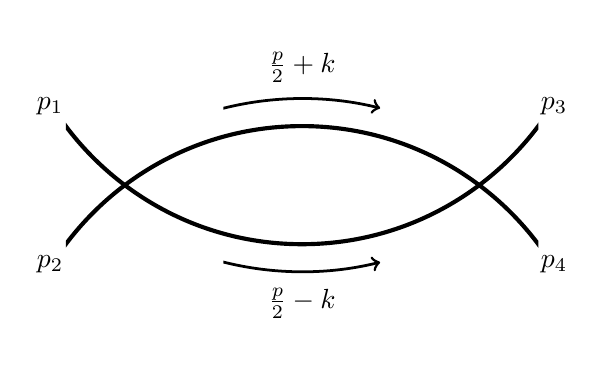
\begin{tikzpicture}[line width=1.5]
		\node at (-3.2, 1) {$p_1$};
		\node at (-3.2, -1) {$p_2$};
		\node at ( 3.2,  1) {$p_3$};
		\node at ( 3.2, -1) {$p_4$};
		\node at (0, 1.5) {$\frac{p}{2}+k$};
		\node at (0,-1.5) {$\frac{p}{2}-k$};
		\clip (-3,-2) rectangle (3,2);
		\draw (0,3) circle (3.75);
		\draw (0,-3) circle (3.75);
		\clip (-1,-2) rectangle (1,2);
		\draw[line width=1,->] (-4.1,3) arc (180:260:4.1) arc (260:284:4.1);
		\draw[line width=1,->] (-4.1,-3) arc (180:100:4.1) arc (100:76:4.1);
	\end{tikzpicture}
\end{center}

\begin{enumerate}

\item Before getting our hands dirty, we should anticipate what's going to happen. Write the appropriate phase space measure $D_{(n)}$ that appears in the `squared amplitude' side of the optical theorem. How many unconstrained momentum integrals are there? Now note that the fish diagram has unconstrained loop momenta. How many $\delta$-functions do we expect to pick up when writing out the imaginary part of the amplitude?

\item Using the momentum assignments above, write out the amplitude for the fish diagram above. We have written $p= p_1+p_2$. Explicitly include factors of $i\epsilon$ since they will be crucial. Do \textit{not} attempt to evaluate the loop momentum integral.

\item Identify the poles in the $k^0$ plane. Work in the center-of-mass frame, $p = (p^0,\mathbf{0})$ and write out the poles to leading order in $\epsilon$. Perform the $dk^0$ integral by closing the integration contour in the lower half and picking up two poles. 

\item Note that performing the $dk^0$ integral via the residue theorem can be recast as replacing one one of the propagators with a $\delta$-function. For each pole write out the appropriate replacement between the propagator and a $\delta$-function. Perform the angular integral and write everything in terms of a single integral over $dE_{\textbf{k}}$ with appropriate integration limits. You may now take $\epsilon\to 0$.

\item  As discussed in class, there is a branch cut in the amplitude when $s=p^2 > 4m^2$. The imaginary part of the amplitude comes from the discontinuity across this cut
$$\text{Disc } A(s) = i \left(\text{Im } A(s+i\varepsilon)-\text{Im } A(s-i\varepsilon)\right) = 2i\text{ Im } A(s+i\varepsilon).$$
This means we can obtain the imaginary part of $A$ by calculating the discontinuity across the cut. Consider the integration contour along the $E_\textbf{k}$ plane. The pole along the imaginary axis can henceforth be ignored. However, the pole along the real axis knows about the branch cut: when $p^0<2m$ it avoids the $dE_\textbf{k}$ contour, whereas for $p^0>2m$ it sits on the contour\footnote{To be technically correct one should say that we started with $p^0<2m$ when we wrote the $dE_\textbf{k}$ contour and are now analytically continuing the function to $p^0>2m$.}. Now calculate the discontinuity by giving $p^2$ a small imaginary part $\pm i\varepsilon$ and calculating the discontinuity. \textit{Hint: use}
$$
\frac{1}{x+i\epsilon} - \frac{1}{x-i\epsilon} = -2\pi i\delta(x).
$$
Note that $\varepsilon$ has nothing to do with the $\epsilon$ in the Feynman propagator. 
Just as in (d) you can recast this as a substitution where one replaces one of the original propagators with a $\delta$-function. Write out this replacement rule explicitly. 

\item Go back to the original amplitude in (b). Write $\int \dbar^4 k = \int \dbar^4q_1 \, \dbar^4q_2 \, (2\pi)^4 \delta^{(4)}(q_1+q_2-k)$ where $q_{1,2} = p/2 \pm k$. We've shown that the discontinuity of the amplitude is given by replacing the propagators according to the two replacement rules in (d) and (e). Write out the final expression for the imaginary part of the amplitude. 

\item Finally, explicitly write out the `squared amplitude' side of the optical theorem, $2 |\mathbf{p_3}| E_\text{CM} \sigma_{\text{tot}}$. Marvel at how it matches what you found in (f). If not, massage a few factors here and there. If you are off by some prefactors, go back and figure out where you dropped them. 

\end{enumerate}


\vspace{1em}

\item{\bf The optical theorem in $\phi^4$ theory to $\mathcal O(\lambda^2)$, another way} [10 points]

The previous problem was somewhat indirect but allowed us to really use the analytic structure of the theory (in particular, the branch cut when the virtual particles go on shell). Here we will derive the same result more directly by starting with the trick that we introduced in Problem 2f.


\begin{center}
	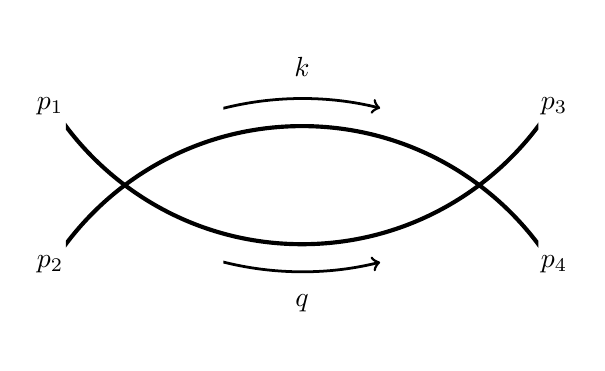
\begin{tikzpicture}[line width=1.5]
		\node at (-3.2, 1) {$p_1$};
		\node at (-3.2, -1) {$p_2$};
		\node at ( 3.2,  1) {$p_3$};
		\node at ( 3.2, -1) {$p_4$};
		\node at (0, 1.5) {$k$};
		\node at (0,-1.5) {$q$};
		\clip (-3,-2) rectangle (3,2);
		\draw (0,3) circle (3.75);
		\draw (0,-3) circle (3.75);
		\clip (-1,-2) rectangle (1,2);
		\draw[line width=1,->] (-4.1,3) arc (180:260:4.1) arc (260:284:4.1);
		\draw[line width=1,->] (-4.1,-3) arc (180:100:4.1) arc (100:76:4.1);
	\end{tikzpicture}
\end{center}

\begin{enumerate}
\item Assign momenta to the fish diagram as shown above. Write out the amplitude as if $d^4k$ and $d^4q$ were two \textit{independent} loop momentum integrals. Insert the appropriate $\delta$-function to make this manifestly equivalent to a single loop integral. Fourier transform this $\delta$-function so that you have an integral over $d^4k\, d^4q\, d^4x$. Note that these loop integrals are in general off shell, that is the $dk^0$ integral is independent of the $dk^i$ integrals.

\item Write the imaginary part of the amplitude as $\text{Im} A = -i (A-A^*)/2$. Evaluate the $dk^0$ and $dq^0$ integrals by taking the appropriate contours. \textit{Hint: if you are getting zero, check overall factors of $i$ in your amplitude.}

\item Confirm that this matches the `squared amplitude' side of the optical theorem. Comment on what happend to the $\delta$-function in (a) after doing the $dk^0$ and $dq^0$ integrals and why this is important for the optical theorem.


\end{enumerate}


\vspace{1em}

\item{\bf Analytic properties in a theory with general masses} [5 points]

Consider a theory with 4 fields $A,B,C,D$ with masses $m_{A,B,C,D}$ and interactions
\[ -\mathcal{L}_I =  \lambda ABC +\lambda A BD.\] 

\begin{enumerate}
\item Draw the Mandelstam-Kibble plot for the $A+A\to C+D$ amplitude. What other amplitudes are related by crossing? Draw and label the kinematic regimes for those other channels on the same Mandelstam-Kibble plot.

\item Sketch the analytic properties expected from unitarity for the $A\to A$ 2-point function.
\end{enumerate}


%\item{\bf The Boltzmann $H$-Theorem} [5 points]
%
%The Boltzmann $H$-theorem is the statement that entropy always increases in an irreversible process. It is often derived in statistical mechanics using the Born approximation or assuming $T$-invariance. Here we will prove it in field theory using unitarity.
%\begin{enumerate}
%
%\item We used $S^\dag S = 1$ to derive the optical theorem. Use $SS^\dag =1$ to prove a very similar relation and hence show that
%$$
%\sum_f \Gamma (a \to f) =  \sum_f \Gamma (f \to a).
%$$
%\item Let $P_i$ be the probability of finding the system in a state $i$. The rate of decrease in $P_i$ due to transitions to other states is $P_i \sum_f \Gamma(i\to f)$ while the rate of increase of $P_i$ due to transitions from all other states is $\sum_f P_f \Gamma(f\to i)$. Show that $\sum_i P_i$ is time-independent. 
%
%\item Entropy is defined as $S = -\sum_i P_i \ln P_i$. Write out the rate of change of entropy. By judicious relabeling of variables, show that this may be written as
%$$
%\frac{dS}{dt} = \sum_{i,f} P_f \ln\left(\frac{P_f}{P_i}\right) \Gamma(f\to i).
%$$
%
%\item Use the inequality
%$$
%y\ln\frac yx \geq y-x
%$$
%and the result of (a) to show that $dS/dt \geq 0$.
%
%
%\end{enumerate}



\end{enumerate}
 

\end{document}
